\documentclass[a4paper,12pt]{article}
\usepackage[top=2cm,bottom=2cm,left=2.5cm,right=1.5cm]{geometry}
\usepackage{fontspec}
\usepackage{polyglossia}
\setmainlanguage{russian}
\IfFontExistsTF{Times New Roman}{%
  \setmainfont{Times New Roman}[Ligatures=TeX]%
  \newfontfamily\cyrillicfont{Times New Roman}[Ligatures=TeX]%
}{\IfFontExistsTF{CMU Serif}{%
  \setmainfont{CMU Serif}[Ligatures=TeX]%
  \newfontfamily\cyrillicfont{CMU Serif}[Ligatures=TeX]%
}{}}
\IfFontExistsTF{Courier New}{%
  \setmonofont{Courier New}%
  \newfontfamily\cyrillicfonttt{Courier New}%
}{\IfFontExistsTF{CMU Typewriter Text}{%
  \setmonofont{CMU Typewriter Text}%
  \newfontfamily\cyrillicfonttt{CMU Typewriter Text}%
}{}}
\usepackage{amsmath,amssymb}
\usepackage{float}
\usepackage{graphicx}
\usepackage{array}
\usepackage{setspace}
\setstretch{1.1}
\setlength{\parindent}{0pt}
\setlength{\parskip}{4pt}
\renewcommand{\arraystretch}{1.25}
\setlength{\tabcolsep}{4.5pt}

\begin{document}

\begin{center}
{\large\bfseries Лабораторная работа\\[2pt]
Решение задачи линейного программирования симплекс-методом}\\[4pt]
Дисциплина: Методы оптимизации
\end{center}

\begin{tabular}{@{}ll}
Ф.И.О.: & Артемов Илья Витальевич\\
Поток: & 1.1\\
Вариант задания: & 1\\
\end{tabular}

\section{Постановка задачи}

Вариант 1. Максимизировать
\[
Z = 2x_1 + 3x_2 + x_3 + 4x_4
\]
при условиях
\[
\left\{
\begin{array}{rcrcrcrcr}
x_1 &+& x_2 &+& x_3 &+& x_4 &\le& 10,\\
2x_1 &+& x_2 &-& x_3 &+& x_4 &=& 8,\\
 & & x_2 &+& 2x_3 &+& x_4 &\ge& 5.
\end{array}
\right.
\]

Задача решается двухфазным симплекс-методом (методом искусственного базиса): сначала вспомогательная задача находит начальный допустимый базисный план, затем решается основная задача.

\textbf{Правила, по которым составлены симплекс-таблицы.}
\begin{itemize}
\item $c_{\text{Б}}$ - коэффициенты целевой функции при базисных переменных, $b$ - значения базисных переменных.
\item Оценки $\Delta_j = \sum_i c_{\text{Б},i}\,a_{ij} - c_j$; в столбце $b$ стоит $\Delta_0 = \sum_i c_{\text{Б},i}\,b_i$, то есть значение целевой функции на текущем плане.
\item Для задачи на максимум план оптимален, если все $\Delta_j \ge 0$.
\item Если есть $\Delta_j < 0$, в базис вводится переменная с наименьшей $\Delta_j$ (при равенстве - с меньшим номером). Из базиса выводится переменная с наименьшим отношением $b_i/a_{ik}$ среди строк с $a_{ik} > 0$. Ведущий элемент выделен рамкой.
\item Пересчёт: ведущая строка делится на ведущий элемент, затем из остальных строк вычитается ведущая, умноженная на соответствующий элемент ведущего столбца.
\end{itemize}

\section{Ход решения}

\subsection*{Шаг 1. Приведение к каноническому виду}

Первое ограничение - неравенство «$\le$»: добавляем к его левой части дополнительную переменную $x_5 \ge 0$. Третье - неравенство «$\ge$»: вычитаем из левой части дополнительную переменную $x_6 \ge 0$. Правые части $b = (10,\ 8,\ 5)$ неотрицательны. Каноническая задача:
\[
Z = 2x_1 + 3x_2 + x_3 + 4x_4 + 0\cdot x_5 + 0\cdot x_6 \to \max,
\]
\[
\left\{
\begin{aligned}
x_1 + x_2 + x_3 + x_4 + x_5 &= 10,\\
2x_1 + x_2 - x_3 + x_4 &= 8,\\
x_2 + 2x_3 + x_4 - x_6 &= 5,
\end{aligned}
\right.
\qquad x_j \ge 0,\ j = 1,\dots,6.
\]

\subsection*{Шаг 2. Вспомогательная задача}

В первом уравнении переменная $x_5$ входит с коэффициентом $1$ и не входит в остальные уравнения, поэтому она может быть базисной. Во втором и третьем уравнениях такой переменной нет ($x_6$ входит с коэффициентом $-1$), поэтому вводим искусственные переменные $y_1, y_2 \ge 0$. Вспомогательная задача:
\[
F = -y_1 - y_2 \to \max \quad(\text{то же, что } y_1 + y_2 \to \min),
\]
\[
\left\{
\begin{aligned}
x_1 + x_2 + x_3 + x_4 + x_5 &= 10,\\
2x_1 + x_2 - x_3 + x_4 + y_1 &= 8,\\
x_2 + 2x_3 + x_4 - x_6 + y_2 &= 5,
\end{aligned}
\right.
\qquad x_j \ge 0,\ y_i \ge 0.
\]
Начальный базис $(x_5, y_1, y_2)$, начальный план $(0,0,0,0,10,0,8,5)$ допустим для вспомогательной задачи.

Если окажется $\max F = 0$ и искусственные переменные выйдут из базиса, получим допустимый базисный план исходной задачи. Если $\max F < 0$, система ограничений несовместна: область допустимых решений пуста и решений нет.

\subsection*{Шаг 3. Решение вспомогательной задачи}

\textbf{Таблица 1.} Для $c_{\text{Б}} = (0,-1,-1)$:
$\Delta_0 = -8-5 = -13$; $\Delta_1 = -2$; $\Delta_2 = -1-1 = -2$; $\Delta_3 = 1-2 = -1$; $\Delta_4 = -1-1 = -2$; $\Delta_5 = 0$; $\Delta_6 = 1$; $\Delta_{y_1} = \Delta_{y_2} = 0$.
Наименьшая оценка $-2$ встречается трижды ($x_1, x_2, x_4$); берём $x_1$ (меньший номер). Отношения: $10/1 = 10$, $8/2 = 4$; в строке $y_2$ элемент равен $0$ и не рассматривается. Минимум $4$ - из базиса выходит $y_1$, ведущий элемент $2$.

\begin{table}[H]
\centering\small
\caption{Вспомогательная задача, начальная таблица}
\begin{tabular}{|c|c|r|r|r|r|r|r|r|r|r|}
\hline
Базис & $c_{\text{Б}}$ & $b$ & $x_{1}$ & $x_{2}$ & $x_{3}$ & $x_{4}$ & $x_{5}$ & $x_{6}$ & $y_{1}$ & $y_{2}$ \\ \hline
$x_{5}$ & $0$ & $10$ & $1$ & $1$ & $1$ & $1$ & $1$ & $0$ & $0$ & $0$ \\
$y_{1}$ & $-1$ & $8$ & $\boxed{2}$ & $1$ & $-1$ & $1$ & $0$ & $0$ & $1$ & $0$ \\
$y_{2}$ & $-1$ & $5$ & $0$ & $1$ & $2$ & $1$ & $0$ & $-1$ & $0$ & $1$ \\
\hline
$\Delta$ & & $-13$ & $-2$ & $-2$ & $-1$ & $-2$ & $0$ & $1$ & $0$ & $0$ \\ \hline
\end{tabular}
\end{table}

\textbf{Таблица 2.} Переменная $y_1$ вышла из базиса, её столбец больше не нужен и отброшен. Для $c_{\text{Б}} = (0,0,-1)$: $\Delta_0 = -5$; $\Delta_2 = -1$; $\Delta_3 = -2$; $\Delta_4 = -1$; $\Delta_6 = 1$; остальные $\Delta_j = 0$. Вводим $x_3$ ($\Delta_3 = -2$). Отношения: $6/1{,}5 = 4$; в строке $x_1$ элемент $-0{,}5 < 0$ не рассматривается; $5/2 = 2{,}5$. Минимум $2{,}5$ - из базиса выходит $y_2$, ведущий элемент $2$.

\begin{table}[H]
\centering\small
\caption{Вспомогательная задача, первая итерация}
\begin{tabular}{|c|c|r|r|r|r|r|r|r|r|}
\hline
Базис & $c_{\text{Б}}$ & $b$ & $x_{1}$ & $x_{2}$ & $x_{3}$ & $x_{4}$ & $x_{5}$ & $x_{6}$ & $y_{2}$ \\ \hline
$x_{5}$ & $0$ & $6$ & $0$ & $0{,}5$ & $1{,}5$ & $0{,}5$ & $1$ & $0$ & $0$ \\
$x_{1}$ & $0$ & $4$ & $1$ & $0{,}5$ & $-0{,}5$ & $0{,}5$ & $0$ & $0$ & $0$ \\
$y_{2}$ & $-1$ & $5$ & $0$ & $1$ & $\boxed{2}$ & $1$ & $0$ & $-1$ & $1$ \\
\hline
$\Delta$ & & $-5$ & $0$ & $-1$ & $-2$ & $-1$ & $0$ & $1$ & $0$ \\ \hline
\end{tabular}
\end{table}

\textbf{Таблица 3.} Все $\Delta_j = 0$, то есть $\Delta_j \ge 0$, план оптимален: $\max F = \Delta_0 = 0$, обе искусственные переменные вне базиса. Получен допустимый базисный план исходной задачи: $x_1 = 5{,}25$, $x_3 = 2{,}5$, $x_5 = 2{,}25$, остальные переменные равны нулю.

\begin{table}[H]
\centering\small
\caption{Вспомогательная задача, оптимальная таблица}
\begin{tabular}{|c|c|r|r|r|r|r|r|r|}
\hline
Базис & $c_{\text{Б}}$ & $b$ & $x_{1}$ & $x_{2}$ & $x_{3}$ & $x_{4}$ & $x_{5}$ & $x_{6}$ \\ \hline
$x_{5}$ & $0$ & $2{,}25$ & $0$ & $-0{,}25$ & $0$ & $-0{,}25$ & $1$ & $0{,}75$ \\
$x_{1}$ & $0$ & $5{,}25$ & $1$ & $0{,}75$ & $0$ & $0{,}75$ & $0$ & $-0{,}25$ \\
$x_{3}$ & $0$ & $2{,}5$ & $0$ & $0{,}5$ & $1$ & $0{,}5$ & $0$ & $-0{,}5$ \\
\hline
$\Delta$ & & $0$ & $0$ & $0$ & $0$ & $0$ & $0$ & $0$ \\ \hline
\end{tabular}
\end{table}

\subsection*{Шаг 4. Переход к основной задаче}

Так как $\max F = 0$ и $y_1, y_2$ не в базисе, переход к основной задаче возможен. Столбцы искусственных переменных отброшены, целевая функция возвращена исходная, $c = (2,3,1,4,0,0)$. Коэффициенты таблицы 3 остаются прежними, базис $(x_5, x_1, x_3)$, $c_{\text{Б}} = (0,2,1)$; пересчитываются только оценки:
\begin{align*}
\Delta_0 &= 2\cdot 5{,}25 + 1\cdot 2{,}5 = 13,\\
\Delta_2 &= 2\cdot 0{,}75 + 1\cdot 0{,}5 - 3 = -1,\\
\Delta_4 &= 2\cdot 0{,}75 + 1\cdot 0{,}5 - 4 = -2,\\
\Delta_6 &= 2\cdot(-0{,}25) + 1\cdot(-0{,}5) - 0 = -1,
\end{align*}
а $\Delta_1 = \Delta_3 = \Delta_5 = 0$ (базисные переменные).

\subsection*{Шаг 5. Решение основной задачи}

\textbf{Таблица 4.} Наименьшая оценка $\Delta_4 = -2$, вводим $x_4$. Отношения: в строке $x_5$ элемент $-0{,}25 < 0$ не рассматривается; $5{,}25/0{,}75 = 7$; $2{,}5/0{,}5 = 5$. Минимум $5$ - из базиса выходит $x_3$, ведущий элемент $0{,}5$.

\begin{table}[H]
\centering\small
\caption{Основная задача, начальная таблица}
\begin{tabular}{|c|c|r|r|r|r|r|r|r|}
\hline
Базис & $c_{\text{Б}}$ & $b$ & $x_{1}$ & $x_{2}$ & $x_{3}$ & $x_{4}$ & $x_{5}$ & $x_{6}$ \\ \hline
$x_{5}$ & $0$ & $2{,}25$ & $0$ & $-0{,}25$ & $0$ & $-0{,}25$ & $1$ & $0{,}75$ \\
$x_{1}$ & $2$ & $5{,}25$ & $1$ & $0{,}75$ & $0$ & $0{,}75$ & $0$ & $-0{,}25$ \\
$x_{3}$ & $1$ & $2{,}5$ & $0$ & $0{,}5$ & $1$ & $\boxed{0{,}5}$ & $0$ & $-0{,}5$ \\
\hline
$\Delta$ & & $13$ & $0$ & $-1$ & $0$ & $-2$ & $0$ & $-1$ \\ \hline
\end{tabular}
\end{table}

\textbf{Таблица 5.} $\Delta_6 = -3$ - вводим $x_6$. Отношения: $3{,}5/0{,}5 = 7$; $1{,}5/0{,}5 = 3$; в строке $x_4$ элемент $-1 < 0$ не рассматривается. Минимум $3$ - из базиса выходит $x_1$, ведущий элемент $0{,}5$.

\begin{table}[H]
\centering\small
\caption{Основная задача, первая итерация ($\Delta_0 = 23$)}
\begin{tabular}{|c|c|r|r|r|r|r|r|r|}
\hline
Базис & $c_{\text{Б}}$ & $b$ & $x_{1}$ & $x_{2}$ & $x_{3}$ & $x_{4}$ & $x_{5}$ & $x_{6}$ \\ \hline
$x_{5}$ & $0$ & $3{,}5$ & $0$ & $0$ & $0{,}5$ & $0$ & $1$ & $0{,}5$ \\
$x_{1}$ & $2$ & $1{,}5$ & $1$ & $0$ & $-1{,}5$ & $0$ & $0$ & $\boxed{0{,}5}$ \\
$x_{4}$ & $4$ & $5$ & $0$ & $1$ & $2$ & $1$ & $0$ & $-1$ \\
\hline
$\Delta$ & & $23$ & $0$ & $1$ & $4$ & $0$ & $0$ & $-3$ \\ \hline
\end{tabular}
\end{table}

\textbf{Таблица 6.} $\Delta_3 = -5$ - вводим $x_3$. Отношения: $2/2 = 1$; в строках $x_6$ и $x_4$ элементы $-3$ и $-1$ отрицательны и не рассматриваются. Из базиса выходит $x_5$, ведущий элемент $2$.

\begin{table}[H]
\centering\small
\caption{Основная задача, вторая итерация ($\Delta_0 = 32$)}
\begin{tabular}{|c|c|r|r|r|r|r|r|r|}
\hline
Базис & $c_{\text{Б}}$ & $b$ & $x_{1}$ & $x_{2}$ & $x_{3}$ & $x_{4}$ & $x_{5}$ & $x_{6}$ \\ \hline
$x_{5}$ & $0$ & $2$ & $-1$ & $0$ & $\boxed{2}$ & $0$ & $1$ & $0$ \\
$x_{6}$ & $0$ & $3$ & $2$ & $0$ & $-3$ & $0$ & $0$ & $1$ \\
$x_{4}$ & $4$ & $8$ & $2$ & $1$ & $-1$ & $1$ & $0$ & $0$ \\
\hline
$\Delta$ & & $32$ & $6$ & $1$ & $-5$ & $0$ & $0$ & $0$ \\ \hline
\end{tabular}
\end{table}

\textbf{Таблица 7.} Все оценки $\Delta_j \ge 0$ ($\Delta_1 = 3{,}5$, $\Delta_2 = 1$, $\Delta_5 = 2{,}5$, остальные нули), план оптимален. Оценки небазисных переменных $x_1, x_2, x_5$ строго положительны, поэтому оптимальный план единственный. Базисные переменные: $x_3 = 1$, $x_6 = 6$, $x_4 = 9$; небазисные $x_1 = x_2 = x_5 = 0$.

\begin{table}[H]
\centering\small
\caption{Основная задача, оптимальная таблица}
\begin{tabular}{|c|c|r|r|r|r|r|r|r|}
\hline
Базис & $c_{\text{Б}}$ & $b$ & $x_{1}$ & $x_{2}$ & $x_{3}$ & $x_{4}$ & $x_{5}$ & $x_{6}$ \\ \hline
$x_{3}$ & $1$ & $1$ & $-0{,}5$ & $0$ & $1$ & $0$ & $0{,}5$ & $0$ \\
$x_{6}$ & $0$ & $6$ & $0{,}5$ & $0$ & $0$ & $0$ & $1{,}5$ & $1$ \\
$x_{4}$ & $4$ & $9$ & $1{,}5$ & $1$ & $0$ & $1$ & $0{,}5$ & $0$ \\
\hline
$\Delta$ & & $37$ & $3{,}5$ & $1$ & $0$ & $0$ & $2{,}5$ & $0$ \\ \hline
\end{tabular}
\end{table}

\subsection*{Шаг 6. Ответ}

Оптимальная точка и значение целевой функции в ней:
\[
x^* = (0,\ 0,\ 1,\ 9)^{\mathsf T} \in X, \qquad Z(x^*) = 2\cdot 0 + 3\cdot 0 + 1 + 4\cdot 9 = 37.
\]
Дополнительные переменные: $x_5^* = 0$, $x_6^* = 6$.

Проверка подстановкой в исходные ограничения:
\begin{align*}
&0 + 0 + 1 + 9 = 10 \le 10 \quad(\text{ограничение активно, } x_5 = 0),\\
&2\cdot 0 + 0 - 1 + 9 = 8 = 8,\\
&0 + 2\cdot 1 + 9 = 11 \ge 5 \quad(\text{не активно, } x_6 = 11 - 5 = 6),
\end{align*}
и $x_j \ge 0$. Значение целевой функции на этой точке совпадает с $\Delta_0$ в таблице 7.

\subsection*{Шаг 7. Решение в Google Таблицах (Solver) и сравнение ответов}

Вместо Excel задача решена в Google Таблицах с надстройкой Solver (SolveSheet, метод Simplex LP). Модель на листе: в ячейках B5:E5 стоят переменные $x_1,\dots,x_4$ (изменяемые ячейки, начальные значения $0$); в B6:E6 - коэффициенты целевой функции, в F6 - формула значения $Z$ (ниже); в B7:E9 - коэффициенты ограничений, в F7:F9 - их левые части, в H7:H9 - правые части $10$, $8$, $5$.

\begin{center}
\texttt{F6: =SUMPRODUCT(B6:E6;\$B\$5:\$E\$5)}
\end{center}
(в F7:F9 - такие же формулы для строк 7--9).

Параметры Solver: цель F6, максимум; изменяемые ячейки B5:E5; ограничения \texttt{F7 <= H7}, \texttt{F8 = H8}, \texttt{F9 >= H9}; включена неотрицательность переменных; метод Simplex LP.

Надстройка сообщила, что решение найдено и все ограничения и условия оптимальности выполнены (рис.~\ref{fig:solver}): $x_1 = x_2 = 0$, $x_3 = 1$, $x_4 = 9$, $Z = 37$; левые части ограничений равны $10$, $8$, $11$.

\begin{figure}[H]
\centering
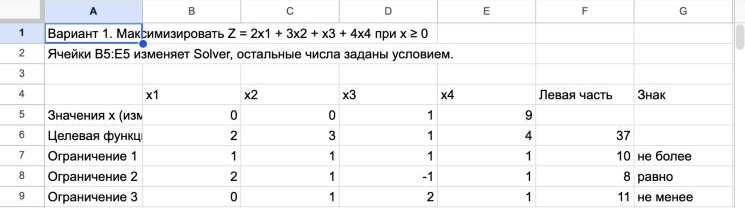
\includegraphics[width=0.8\textwidth]{screenshots/solver_sheet.png}\\[6pt]
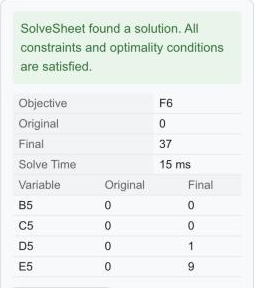
\includegraphics[width=0.30\textwidth]{screenshots/solver_report.png}
\caption{Результат Solver: таблица с найденными значениями (вверху) и отчёт надстройки (внизу)}
\label{fig:solver}
\end{figure}

\begin{table}[!htbp]
\centering
\caption{Сравнение ответов}
\begin{tabular}{|l|c|c|}
\hline
Способ решения & Оптимальная точка $x^*$ & $Z(x^*)$\\ \hline
Симплекс-метод (таблицы 1--7) & $(0,\ 0,\ 1,\ 9)$ & $37$\\ \hline
Solver (Google Таблицы, Simplex LP) & $(0,\ 0,\ 1,\ 9)$ & $37$\\ \hline
\end{tabular}
\end{table}
Ответы совпадают.

\section{Рефлективный вывод}

\textbf{Что оказалось полезным.} Работа показала весь путь решения задачи линейного программирования: от системы с неравенствами и равенством к канонической форме, затем поиск начального допустимого плана через вспомогательную задачу и только потом оптимизация.

\textbf{Трудности и как они преодолевались.}
\begin{enumerate}
\item В условии не записана неотрицательность переменных. Я принял стандартное допущение $x_j \ge 0$ и явно указал его в постановке.
\item В таблице 1 наименьшая оценка $-2$ встречается трижды, так что правило выбора ведущего столбца неоднозначно. Я зафиксировал правило «наименьшая $\Delta_j$, при равенстве - меньший номер» и применял его во всех таблицах.
\item В таблицах много дробей (четверти) и знаков, при пересчёте легко ошибиться. После каждой итерации я проверял, что столбцы базисных переменных остались единичными, а $\Delta_0$ равна значению целевой функции на текущем плане, а итоговый ответ подставил в исходные ограничения. Таблицы также сверены с программой на точных дробях (\texttt{simplex.py}) и с результатом \texttt{scipy.optimize.linprog}.
\item Excel на компьютере был без подписки и открывал файлы только для чтения, поэтому надстройка Solver в нём не работала. Проверку я выполнил в Google Таблицах с надстройкой SolveSheet (метод Simplex LP): результат совпал с ручным решением.
\end{enumerate}

\end{document}
